
\documentclass[a4paper]{article}
\usepackage{graphicx}
\usepackage{subcaption}
\usepackage{tikz}
\usepackage{url}
\usepackage{MnSymbol}
\usetikzlibrary{arrows}
\usetikzlibrary{calc}

\usepackage{xcolor}
\usepackage{listings}
\lstset{basicstyle=\ttfamily,
showstringspaces=false,
commentstyle=\color{red},
numbers=left,
linewidth=12.1cm
}

\lstset{breaklines=true, breakatwhitespace=true}
\lstset{prebreak= }
\lstset{postbreak=}


\newcommand{\rospackage}[1]{\textbf{\textit{ros-indigo-#1}}}
\newcommand{\rostopic}[1]{\textbf{\textit{#1}}}
\begin{document}

\title{Implementation of 2d navigation for a moving base using ROS
(version 1.0)
}
\date{\today}
\author{Windel Bouwman}

\maketitle
\begin{abstract}
This document describes the application of navigation software
as available in ROS to the modified x80sv robot. Different ROS
packages were evaluated on the robot.
\end{abstract}

\tableofcontents

\section*{List of symbols}

\begin{tabular}{ | l | l | l | }
  \hline                       
  Symbol & Unit & Description \\
  \hline                       
  $l_{base}$ & $[m]$ & Distance between the two wheels of the robot. \\
  \hline                       
  $r_{wheel}$ & $[m]$ & Radius of the wheel. \\
  \hline                       
  $N_{enc}$ & $[-]$ & Number of pulses per rotation of the encoders \\
  \hline                       
  $v_{max}$ & $[m/s]$ & Maximum forward velocity. \\
  \hline                       
  $a_{max}$ & $[m/s^2]$ & Maximum forward acceleration. \\
  \hline                       
  $\omega_{max}$ & $[rad/s]$ & Rotational maximum velocity. \\
  \hline                       
  $\alpha_{max}$ & $[rad/s^2]$ & Rotational maximum acceleration. \\
  \hline                       
  $v$ & $[m/s]$ & Forward velocity of the robot. \\
  \hline                       
  $\omega$ & $[m/s]$ & Rotational velocity of the robot. \\
  \hline                       
  $\omega_l$ & $[rad/s]$ & Rotational velocity of the left wheel. \\
  \hline                       
  $\omega_r$ & $[rad/s]$ & Rotational velocity of the right wheel. \\
  \hline                       
  $\theta$ & $[rad]$ & Rotation of the robot with respect to the world. \\
  \hline                       
\end{tabular}

\begin{thebibliography}{1}

  \bibitem{gmapping} ROS gmapping \url{http://wiki.ros.org/gmapping}

  \bibitem{x80sv} x80sv software \url{https://github.com/SaxionLED/x80sv}

  \bibitem{globalompl} Ompl plugin
\url{https://github.com/windelbouwman/move-base-ompl}

  \bibitem{ompl} Ompl library \url{http://ompl.kavrakilab.org/}

  \bibitem{amcl} \url{http://wiki.ros.org/amcl}

  \bibitem{tuningguide} \url{http://wiki.ros.org/navigation/Tutorials/Navigation%20Tuning%20Guide}
\end{thebibliography}

\clearpage

\section{Introduction}

This document describes how the problem of 2d-navigation was solved on a real robot.
The goal of navigation is to safely move a robot from a to b.

The task of navigation can be split up into the following tasks (see figure \ref{fig:overview}):

\begin{itemize}
  \item Robot control. This task is concerned with controlling the seperate wheels of the robot.
  Typically this is done using PID control or something alike.
  \item Odometry calculation. By keeping track of wheel motions, the robot position can be
calculated. This method is subjective to drift.
  \item Position and mapping, also known as SLAM, is the task of determining location of the robot in 
  the world, and at the same time reconstructing the world.
  \item Global planning is the task of determining a path through a known map. This requires a search
  like A* or something like that.
  \item Local planning takes as input the global path and generated the appropriate motion commands for
  the robot control. It is some sort of setpoint generator. This layer is also responsible for obstacles.
  When an obstacle is observed, the path may be adjusted.
  \item Semantic interpretation is the process of converting a task into a sequence of locations to be
  reached. For example the conversion of the sentence "fetch beer" into a path from the current location
  to nearest fridge.
\end{itemize}

\begin{figure}
  \centering

% Usage of the ticks package:
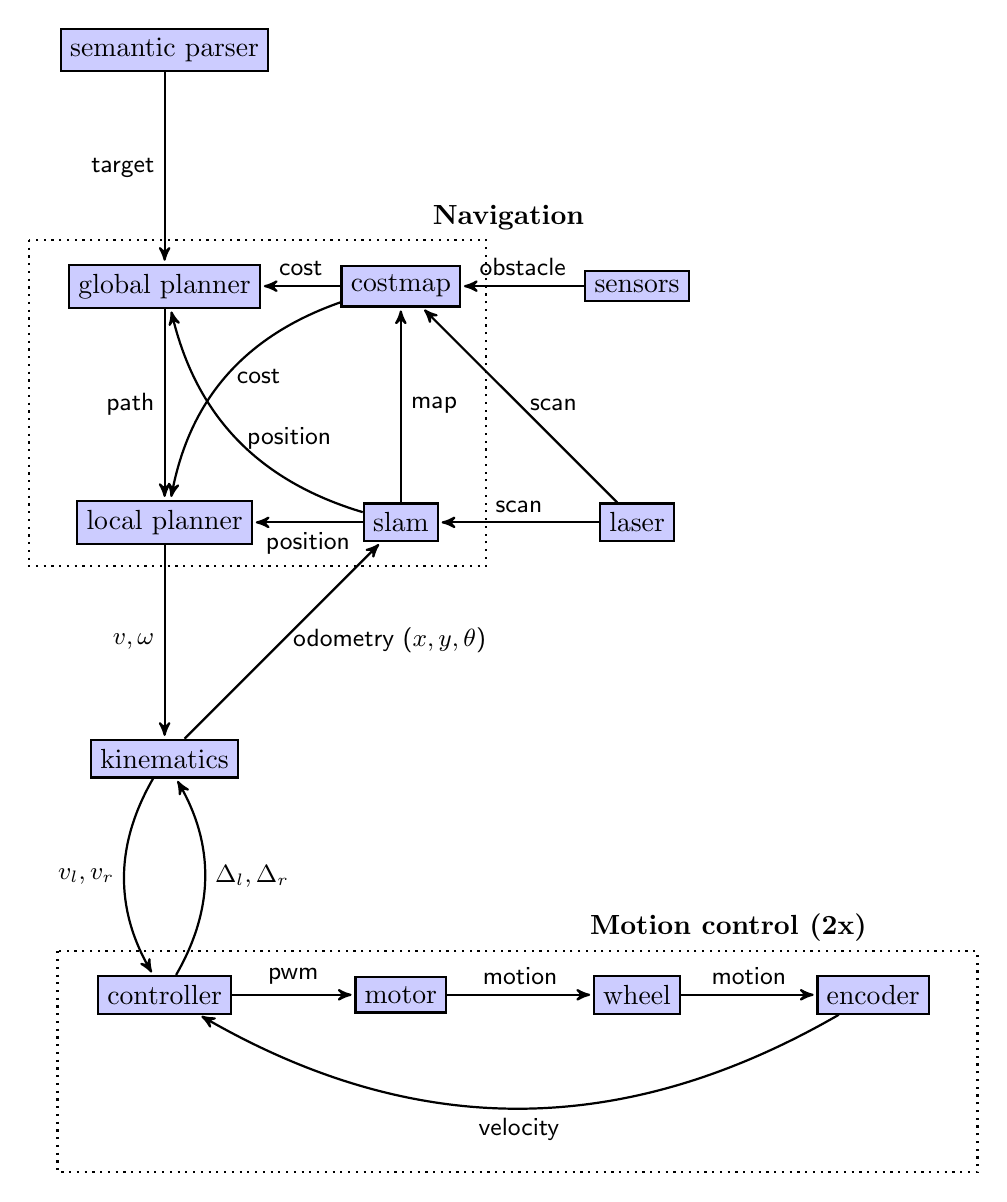
\begin{tikzpicture}[->,>=stealth',shorten >=1pt,auto,node distance=3cm,
  thick,main node/.style={rectangle,fill=blue!20,draw}]

  \node[main node] (C) {controller};
  \node[main node] (2) [right of=C] {motor};
  \node[main node] (3) [right of=2] {wheel};
  \node[main node] (4) [right of=3] {encoder};
  \node[main node] (KIN) [above of=C] {kinematics};
  \node[main node] (5) [above of=KIN] {local planner};
  \node[main node] (GP) [above of=5] {global planner};
  \node[main node] (7) [right of=5] {slam};
  \node[main node] (8) [right of=7] {laser};
  \node[main node] (9) [above of=GP] {semantic parser};
  \node[main node] (10) [above of=7] {costmap};
  \node[main node] (11) [above of=8] {sensors};
  
  \draw[thick,dotted]     ($(GP.north west)+(-0.5,0.3)$) rectangle ($(7.south east)+(0.6,-0.3)$);
  \node[font=\bf] at ($(10.north east)+(0.6,0.6) $) {Navigation};

  \draw[thick,dotted]     ($(C.north west)+(-0.5,0.3)$) rectangle ($(4.south east)+(0.6,-2.0)$);
  \node[font=\bf] at ($(3.north east)+(0.6,0.6) $) {Motion control (2x)};

  \path[every node/.style={font=\sffamily\small}]
    (C) edge node [above] {pwm} (2)
    (2) edge node [above] {motion} (3)
    (3) edge node[above] {motion} (4)
    (4) edge [bend left] node [below] {velocity} (C)
    (5) edge node [left] { $v,\omega$} (KIN)
    (KIN) edge [bend right] node [left] { $ v_l, v_r $ } (C)
    (C) edge [bend right] node [right] { $ \Delta_l, \Delta_r $ } (KIN)
    (GP) edge node [left] {path} (5)
    (7) edge [bend left] node [right] {position} (GP)
    (7) edge node [below] {position} (5)
    (7) edge node [right] {map} (10)
    (KIN) edge node [right] {odometry ($x,y,\theta$) } (7)
    (8) edge node [above] {scan} (7)
    (8) edge node [right] {scan} (10)
    (9) edge node [left] {target} (GP)
    (10) edge node [above] {cost} (GP)
    (10) edge [bend right] node [right] {cost} (5)
    (11) edge node [above] {obstacle} (10)
    ;
\end{tikzpicture}
  \caption{The building blocks involved in the task of navigation. Inside the rectangle is the core functionality.}
  \label{fig:overview}
\end{figure}


The rest of this document describes all the tasks listed above as applied to the x80sv using
the robot operating system (ROS).

\clearpage

\section{ROS concepts}
\subsection{Basics}
ROS is a robotic operation system. Is provides infrastructure to build robot applications.
A ROS system consists of nodes, these are running programs performing some task. Nodes can
interchange data via topics via a publish subscribe mechanism. Other concepts are services
and parameters.

\subsection{Rviz}
Rviz is an indispensible tool when debugging a robotic system. With rviz one can visualize a robot
and its environment. The tool consists of a main window and a pane to the left where various data
visualizers can be added.

\subsection{Rqt}
Another helpful tool when debugging a ros system is rqt. This tool is a plugin container where plugins
can be selected. Plugins exists for tf tree visualization, node interconnect, topic inspection,
logging viewer, diagnostics viewer and more.

\subsection{Tf}
The tf (\url{http://wiki.ros.org/tf}) system of ROS is used to describe the various parts of 
a robot in space. The TF-tree of a robot is the relative position of all bodies of a robot
with respect to eachother.

\subsection{Gazebo}
Gazebo is a physics simulator, which can be in combination with ROS. In gazebo entire worlds
can be modelled. In this world, all kind of objects can be inserted. For example a motor can
be inserted, which is coupled with a ROS topic. Gazebo is a physics simulator, so every friction
and contact force can be modelled.

\subsection{Urdf}
To describe robotic systems in ROS the urdf file format is used. An urdf file is a xml file
with tags describing links and joints of a robot. The file format can be used by both gazebo
and rviz. It also contains information about how a robot must be visualized by textures, shapes
and colors. The physical parameters are also described with this file.

To simplify the writing of urdf, the macro language xacro can be used. Xacro files can be
automatically expanded into urdf files via the xacro script. Usually this is done when the
urdf is loaded.

\section{Robot setup}
The robot used in this setup is the x80sv of drrobot. This robot has three wheels, of which
two are controlled. Other sensors are range sensors, infrared and ultrasonic.
The robot is extended with a laser range
sensor (LRS) and a laptop with ROS installed. The LRS and the controllerboard of the x80sv are
connected via usb-serial cables. The controllerboard of the x80sv is provided with
the robot.

\begin{figure}[h!]
  \centering
  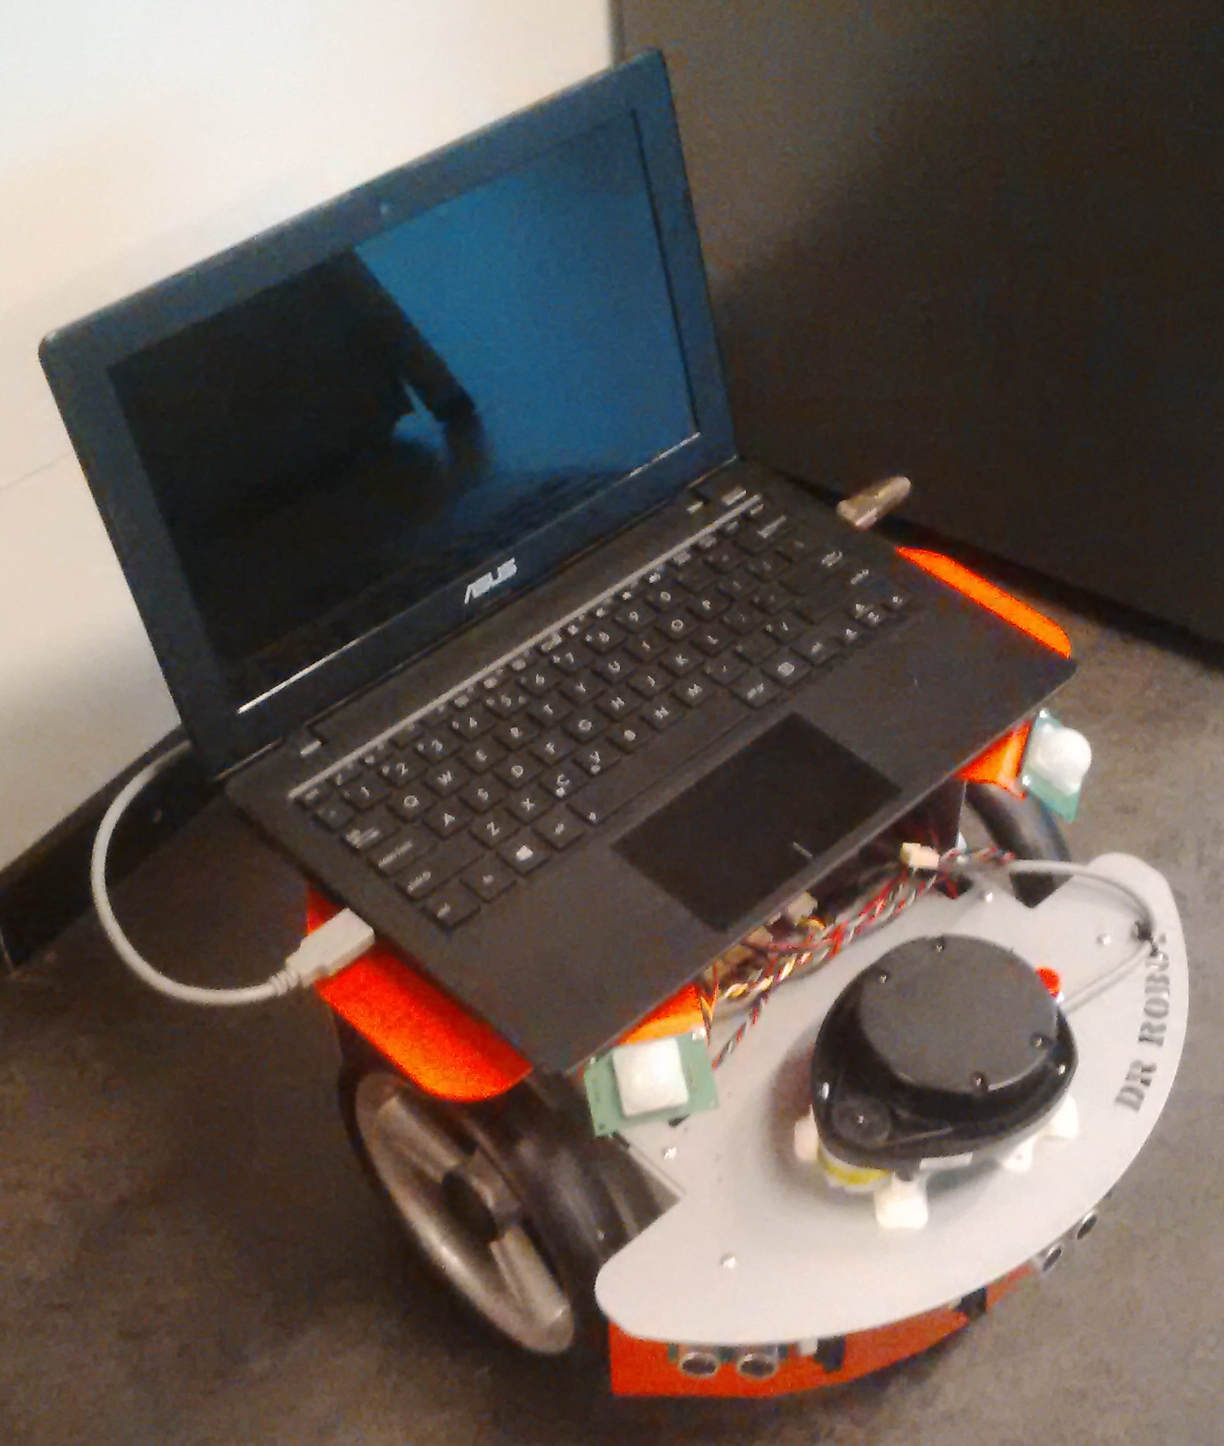
\includegraphics[width=\textwidth,height=\textheight,keepaspectratio]{img/fotorobot.png}
  \caption{Photo of the x80sv equiped with laptop and LRS}
\end{figure}

\begin{tabular}{ | l | l | l |}
  \hline                       
  Parameter & Value & Description\\
  \hline 
  \hline 
  $N_{enc}$ & 756 [-] & Encoder ticks per wheel revolution \\
  \hline
  $r_{wheel}$ & 0.085 [m] & Wheel radius\\
  \hline
  $l_{base}$ & 0.283 [m] & Distance between left and right wheel\\
  \hline
\end{tabular}

\subsection{Installation}
To use the robot, install ROS indigo on ubuntu 14.04 on the robot laptop. Download the 
x80sv software from the github repository \cite{x80sv}. Follow 
instruction in the readme.

\subsection{Robot description}
To use the robot with the ROS system, an urdf model must be created. The model of the x80sv is
located in the folder \url{x80sv_description}. The xacro macro system is used to simplify the
writing of the urdf file. The urdf description contains a description of what links and joints
the robot consists of. The model is used by rviz for visualization and by gazebo to construct
the physical model of the robot to simulate it. The weights, shapes and materials of the links
are also specified in this file.


\subsection{Simulation}
Instead of trying to run everything on the real robot, a simulated version of the x80sv
was created.

With this simulation it is possible to run the exact same navigation software with the real
robot as well as with the simulated variant.

\begin{figure}[h!]
  \centering
  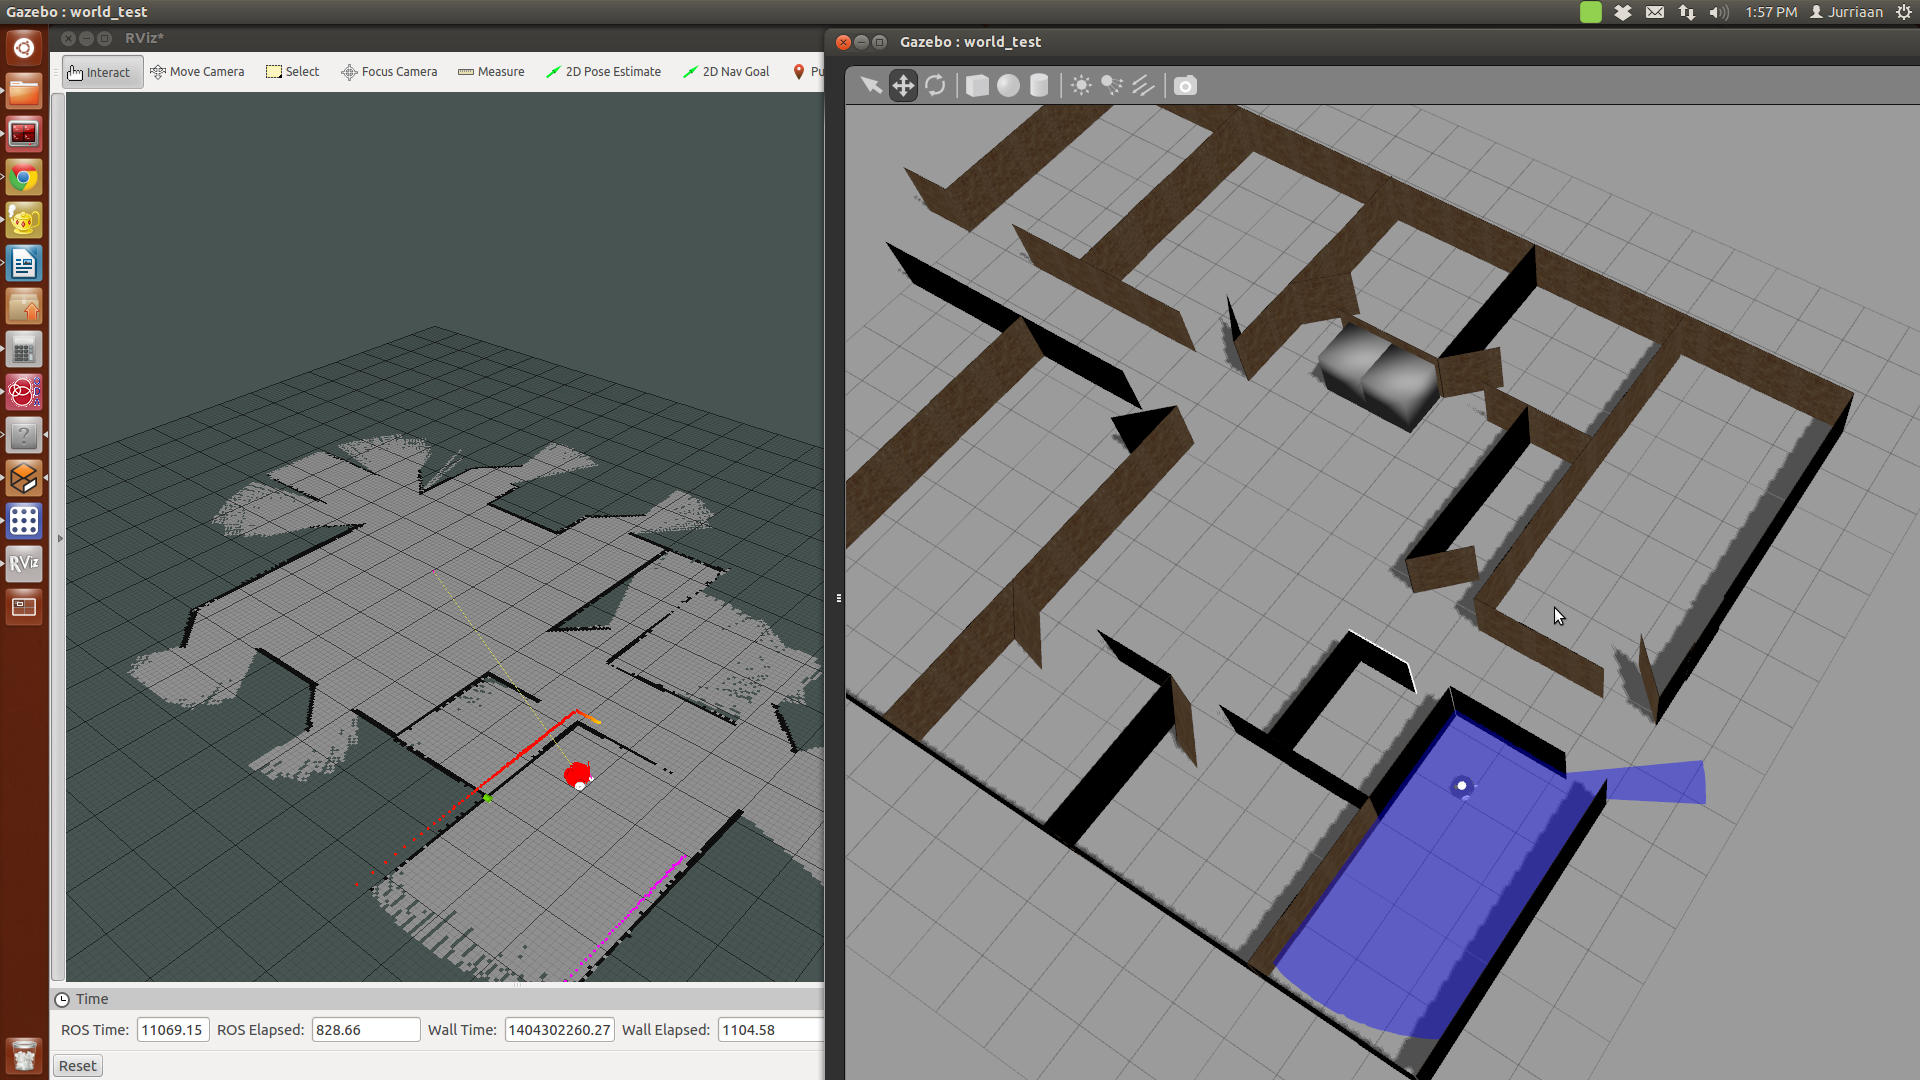
\includegraphics[width=\textwidth,height=\textheight,keepaspectratio]{img/office_sim_testgmapping.png}
  \caption{Gazebo (right) and rviz (left) running a simulated robot}
\end{figure}

\begin{figure}[h!]
  \centering
  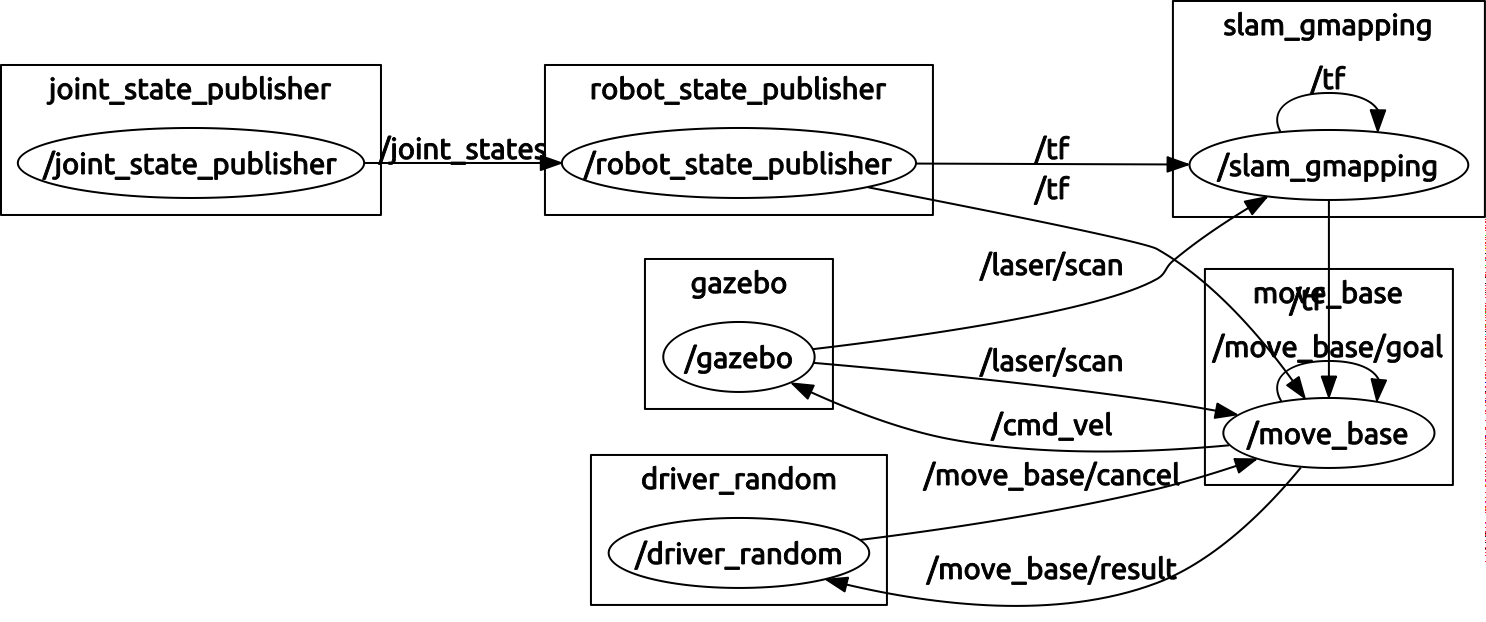
\includegraphics[width=\textwidth,height=\textheight,keepaspectratio]{img/simulatie_nodes.png}
  \caption{The nodes involved in the simulation}
\end{figure}


\section{Navigation on the x80sv}

There is an existing framework for 2d mobile base navigation \url{http://wiki.ros.org/move_base}.
Another framework is the skynav framework developed at saxion \url{https://github.com/SaxionLED/skynav}
Those two should be interchangable. They both publish the \rostopic{cmd\_vel} topic,
subscribe to sensors such as laser, infrared and ultrasonic, and they receive
navigation goals from a higher level module.
For this project the move-base navigation
stack was selected.

\subsection{Kinematics}

Two-wheeled vehicles have the following kinematic equations of motion.
Given $\Delta_{left}$ and $\Delta_{right}$ as the traveled distance for the left and
right wheels, we can calculate the traveled distance forward and rotation.

\begin{figure}[h!]
 \centering
 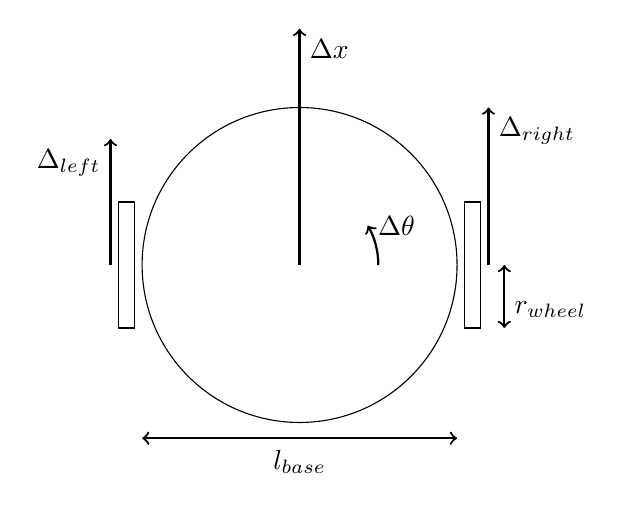
\begin{tikzpicture}
  \draw (0,0) circle (2);
  \draw[thick,->] (0,0) -- (0,3) node[anchor=north west] {$\Delta x$};

  \draw (-2.3,-0.8) rectangle (-2.1,0.8);
  \draw (2.1,-0.8) rectangle (2.3,0.8);
  \draw[thick,->] (-2.4,0) -- (-2.4,1.6) node[anchor=north east] {$\Delta _{left}$};
  \draw[thick,->] (2.4,0) -- (2.4,2) node[anchor=north west] {$\Delta _{right}$};
  \draw[thick,->] (1,0) arc (0:30:1) node[anchor=west] {$\Delta \theta$};
  \draw[thick,<->] (-2,-2.2) -- (2,-2.2);
  \draw[thick,<->] (2.6,0) -- (2.6,-0.8) node[anchor=south west] {$r_{wheel}$};
  \node at (0, -2.5) {$l_{base}$};
 \end{tikzpicture}
 \caption{Robot kinematics}
\end{figure}

\begin{equation}
\Delta x = \frac{\Delta_{left} + \Delta_{right}}{2}
\end{equation}

\begin{equation}
\Delta \theta = tan^{-1}(\frac{\Delta_{right} - \Delta_{left}}{l_{base}})
\end{equation}

Given these traversed deltas we can now compute the new position and orientation
of the robot in world coordinates.
\begin{equation}
 x_{x+1} = x_{n} + \cos(\theta_n) \Delta x
\end{equation}
\begin{equation}
 y_{x+1} = y_{n} + \sin(\theta_n) \Delta x
\end{equation}
\begin{equation}
 \theta_{x+1} = \theta_{n} + \Delta \theta
\end{equation}

\subsubsection{Control}

The velocity control is done by the controllerboard of the robot. The commands to
the controllerboard are wheel velocities in encoder ticks. A conversion from linear
and angular velocities to wheel velocities is required.

\begin{equation}
        \omega_{left} = \frac{v - \frac{1}{2} * \omega * l_{base}}{r_{wheel}}
\end{equation}
\begin{equation}
        \omega_{right} = \frac{\frac{1}{2} * \omega * l_{base} + v}{r_{wheel}}
\end{equation}

In the next step, the wheel velocities are translated into encoder velocities.

\begin{equation}
  leftWheelCmd = \frac{- \omega_{left} * N_{enc}}{2 \pi}
\end{equation}
\begin{equation}
 rightWheelCmd = \frac{\omega_{right} * N_{enc}}{2 \pi}
\end{equation}

These equations are implemented in the real robot drivers (\url{https://github.com/SaxionLED/x80sv/tree/master/x80sv_driver}). In case of simulation, these equations are done by gazebo.

\subsubsection{Odometry}
The task of the odometry system is to keep track of the robot position using wheel encoder
data. To implement this for a two wheeled robot the following formulas are used:

\begin{equation}
 d_{left} = calculateMovementDelta(mtr0)
\end{equation}
\begin{equation}
 d_{right} = calculateMovementDelta(mtr1)
\end{equation}
\begin{equation}
 averageDistance = (d_{left} + d_{right}) / 2
\end{equation}
\begin{equation}
 \delta \theta = atan2((d_{right} - d_{left}), wheelDis_);
\end{equation}
\begin{equation}
 \delta x = averageDistance * cos(\theta);
\end{equation}
\begin{equation}
 \delta y = averageDistance * sin(\theta);
\end{equation}
\begin{equation}
 \theta += \delta \theta
\end{equation}
\begin{equation}
 x += \delta x
\end{equation}
\begin{equation}
 y += \delta y
\end{equation}

These equations are implemented in the real robot drivers (\url{https://github.com/SaxionLED/x80sv/tree/master/x80sv_driver}). In case of simulation, these equations are done by gazebo.

\subsection{Gmapping}

Simultaneous localization and mapping (SLAM), is a required component for navigation.
The task of the SLAM module in a robotic system is determining the robots position
in space, and while doing that, determine a map of the environment. There exist
several packages to do this.

For the x80sv the package \rospackage{gmapping} \cite{gmapping} was used.
This node takes as input the odometry data from the control layer and the laser scan
data. It then is capable of generating a map and determining the drift that occurred
since odometry start.

The tf tree is visualized in figure~\ref{fig:tftreesim}. The map
frame is the world frame. The gmapping node determines the transform between map and odom
frame. The odom frame is the frame in which the robot started to drive. The transform
betweet odom and base footprint is the transform as recorded by the odometry system.
In the case of the simulation, gazebo takes care of this transform. When using the
real robot, the x80 driver records the transformation. From the base footprint the rest
of the mobile base consists of links which have static transforms.

\begin{figure}[h!]
  \centering
  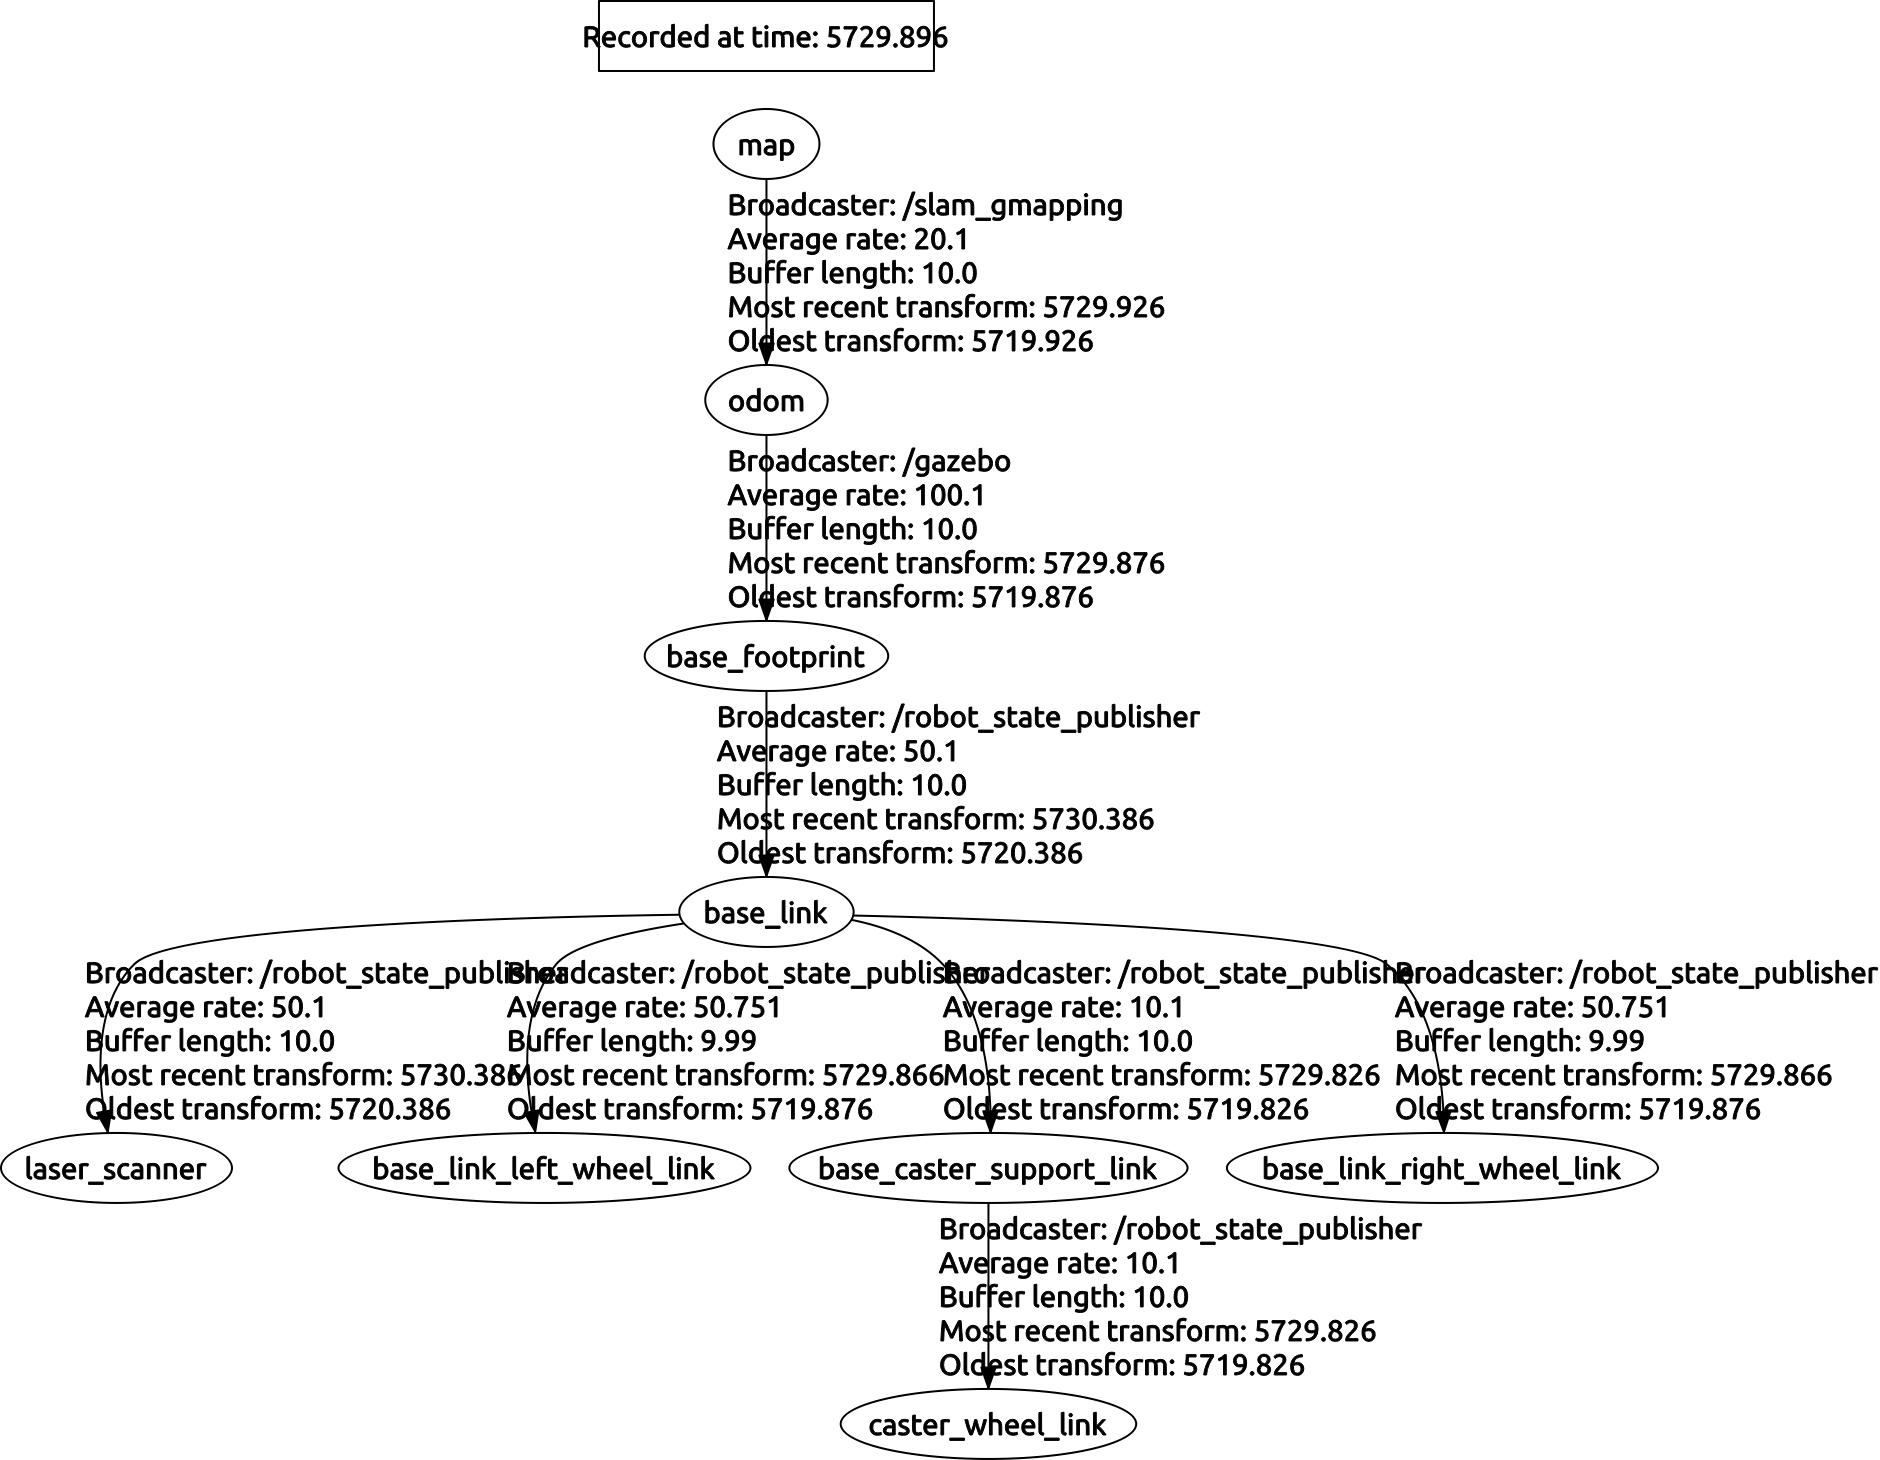
\includegraphics[width=\textwidth,height=\textheight,keepaspectratio]{img/tf_tree_simulation.png}
  \caption{tf tree visualized with rqt tf tree plugin}
  \label{fig:tftreesim}
\end{figure}

\subsubsection{Laser orientation}
The orientation of the laser is important for the gmapping node. The gmapping node assumes that
the scan data is symmetric around zero angle.

This was discovered during experiments with the gmapping node.
The minimum and maximum range
$0 .. 2\pi$ did not work. A range from $-\pi .. \pi$ did work!
The scan data contains the same bytes, but the minimum and maximum angle
as defined in the scan message was adjusted. Also the reference frame
of the laser scanner had to be adjusted. All these changes could be done
without the laser scanner being physically remounted!

These changes also resulted in the simulated and the real robot behave the same.

\begin{figure}[h!]
  \centering
  \begin{subfigure}[b]{0.4\textwidth}
    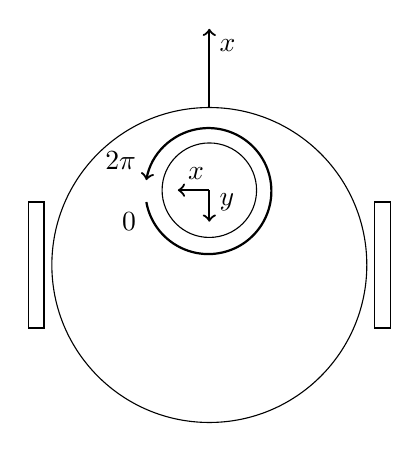
\begin{tikzpicture}
    \draw (0,0) circle (2);
    \draw (0,0.95) circle (0.6);
    \draw[thick,->] (0,2) -- (0,3) node[anchor=north west] {$x$};
    \draw[thick,->] (0,0.95) -- (-0.4,0.95) node[anchor=south west] {$x$};
    \draw[thick,->] (0,0.95) -- (0.0,0.55) node[anchor=south west] {$y$};
    \draw (-2.3,-0.8) rectangle (-2.1,0.8);
    \draw (2.1,-0.8) rectangle (2.3,0.8);
    \draw[thick,->] (-0.8,0.8) arc (190:530:0.8) node[anchor=south east] {$ 2\pi$};
    \draw[thick,-] (-0.8,0.8) arc (190:190:0.8) node[anchor=north east] {$ 0$};
    \end{tikzpicture}
    \caption{Laser orientation and scan angles that did not work}
  \end{subfigure}
  ~~~
  \begin{subfigure}[b]{0.4\textwidth}
    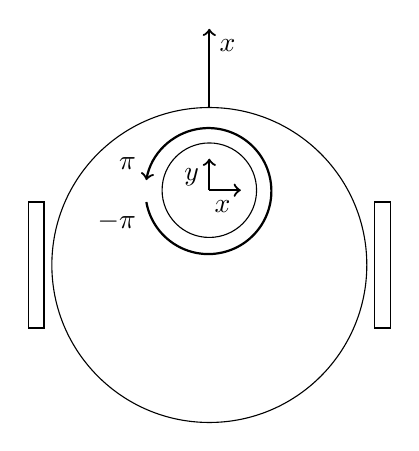
\begin{tikzpicture}
    \draw (0,0) circle (2);
    \draw (0,0.95) circle (0.6);
    \draw[thick,->] (0,2) -- (0,3) node[anchor=north west] {$x$};
    \draw[thick,->] (0,0.95) -- (0.4,0.95) node[anchor=north east] {$x$};
    \draw[thick,->] (0,0.95) -- (0.0,1.35) node[anchor=north east] {$y$};
    \draw (-2.3,-0.8) rectangle (-2.1,0.8);
    \draw (2.1,-0.8) rectangle (2.3,0.8);
    \draw[thick,->] (-0.8,0.8) arc (190:530:0.8) node[anchor=south east] {$ \pi$};
    \draw[thick,-] (-0.8,0.8) arc (190:190:0.8) node[anchor=north east] {$-\pi$};
    \end{tikzpicture}
    \caption{Laser orientation and scan angles that did work}
  \end{subfigure}
  \caption{Laser reference frame and minimum and maximum angles appeared to be important for the gmapping node}
  \label{fig:laserorientation}
\end{figure}

\subsection{Move base}

The \rospackage{move-base} package provides a sort of infrastructure for 2d mobile base
navigation. It provides a structure into which plugins can be inserted.
Among plugins are costmap function, recovery behaviors, local planner and global planner.

\begin{figure}[h!]
  \centering
  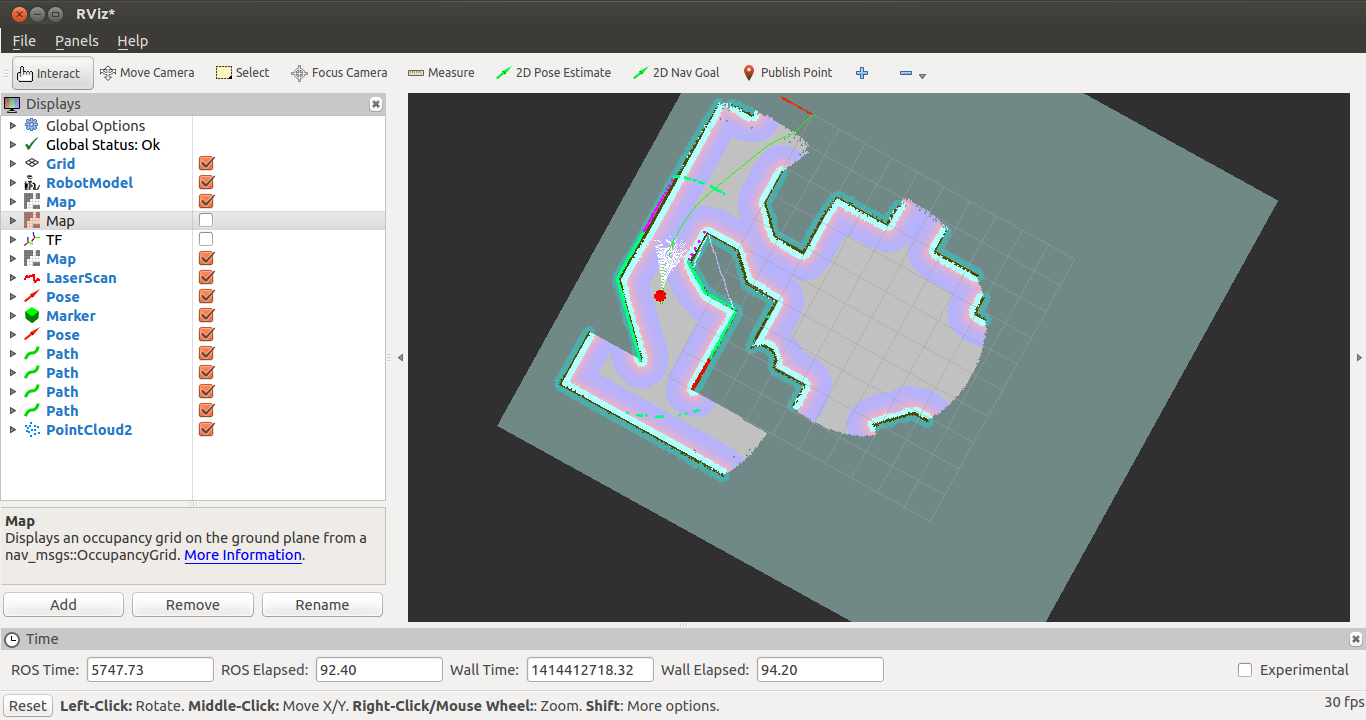
\includegraphics[width=\textwidth,height=\textheight,keepaspectratio]{img/rviz_navigation2.png}
  \caption{Navigation visualized in rviz}
  \label{fig:navrviz}
\end{figure}

\subsection{Costmap2d}
The \rospackage{costmap-2d} is a ros package that can create a costmap of the environment
of the robot.
The costmap is then used by both global and local planning to determine the path.
The costmap consists of several input layers. The static layer takes the map as determined by
gmapping and inflates it somehwat. The obstacle layer can incorporate different sensors.
Rviz can be used to visualize these costmaps.

\subsection{Local planning}
To implement local planning on the x80sv, the navigation tuning guide was followed closely
\cite{tuningguide}.

\subsubsection{Robot physical limits}
In order to perform good navigation, certain robot parameters must be known. These include the
robot maximum acceleration and maximum velocity for both linear and rotational motion. To
Determine this, the robot was driven at its maximum speed, and the velocities as measured by
the encoders was logged. This was done using the ROS x80 driver, see listing \ref{lst:robotlimits}.
At line 1, the real robot driver is launched. The robot can now be controlled via rqt.
Line 2 starts a recording of the odom and cmd\_vel topics into a bag file. Now, the robot
was moved using the robot steering plugin of rqt. At line 3 the rosbag file is converted to
a csv file. Line 4 activates a script that plots the csv file into figure \ref{fig:robotlimits}.

From figure \ref{fig:robotlimits} the following robot limitations are determined:

\begin{tabular}{ | l | l | }
  \hline                       
  Parameter & Value \\
  \hline                       
  \hline                       
  $v_{max}$ & $0.4 [m/s] $ \\
  \hline                       
  $a_{max}$ & $ 1.0 [m/s^2] $\\
  \hline                       
  $\omega_{vmax}$ & $ 2.0 [rad/s] $ \\
  \hline                       
  $\alpha_{max}$ & $ 5.0 [rad/s^2] $ \\
  \hline  
\end{tabular}

\begin{lstlisting}[language=bash,caption={commands to determine robot limitations},
    label=lst:robotlimits]
launch x80sv_bringup real_robot_driver.launch
rosbag record odom cmd_vel
rostopic echo -b 2014-12-01-14-44-27.bag -p /odom/twist > measurement.txt
python3 plot_acceleration.py
\end{lstlisting}


\begin{figure}[h!]
  \centering
  \begin{subfigure}[b]{0.8\textwidth}
    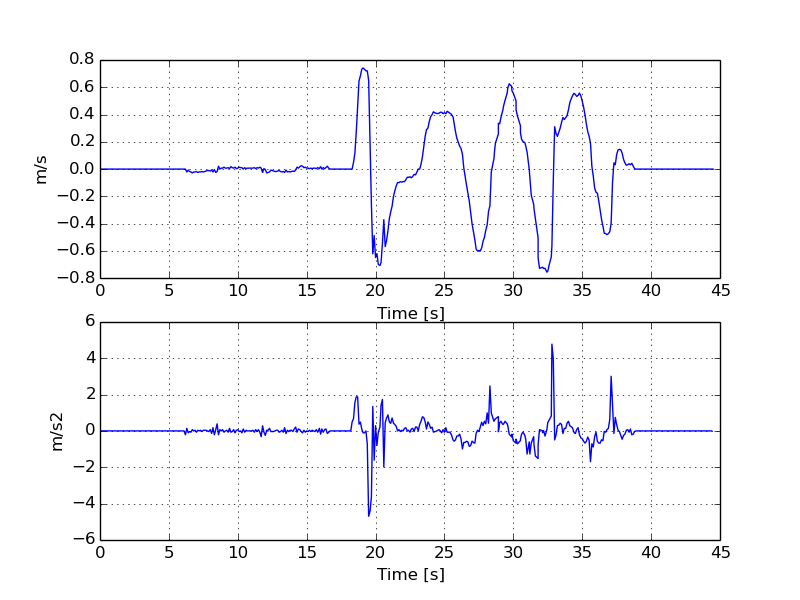
\includegraphics[width=\textwidth,height=\textheight,keepaspectratio]{img/v.png}
    \caption{Measured linear velocity and calculated acceleration}
  \end{subfigure}
  \begin{subfigure}[b]{0.8\textwidth}
    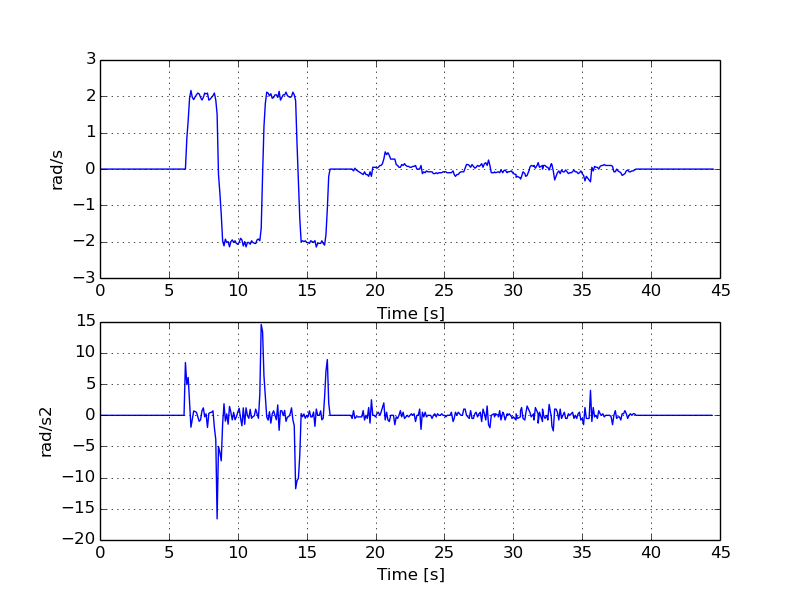
\includegraphics[width=\textwidth,height=\textheight,keepaspectratio]{img/omega.png}
    \caption{Measured rotational velocity and calculated acceleration}
  \end{subfigure}
  \caption{Measured velocities}
  \label{fig:robotlimits}
\end{figure}


\subsubsection{base local planner}
The default planner of the \rospackage{move-base} package for ROS is the base local planner.
This planner uses dynamic window approach (DWA) to plan a path. This means that from the current 
location several path options are simulated in advance and the one with the least cost is selected.
This planner has several parameters that must be tuned to a specific robot.

\subsubsection{DWA local planner}
The dwa local planner is also a standard ROS planner. It is contained in the package
\rospackage{dwa-local-planner}.
It is simpler than the base local planner,
that is why this package is chosen as currently the best solution.

\subsubsection{Smooth planner}
The smooth planner is own work, and is located at github (
\url{https://github.com/SaxionLED/x80sv/tree/master/smooth_local_planner}).
This planner follow the global path and when confronted with an obstacle simply
reports that the plan has failed and waits for new commands from the global planner.
This planner can be extended to include smooth motion profiles to the wheel base.

\subsection{Global planning}

\subsubsection{Global planner}
The \rospackage{global-planner} package contains a global planner that uses simple search
for an optimal path given a costmap. It is a plugin for use with move-base.
This was the global navigation plugin that was used for the x80sv.

\subsubsection{Navfn planner}
The \rospackage{navfn} package provides another plugin for move-base for global navigation.
This is an existing ROS module. It was tried on the x80sv, and is an alternative to \rospackage{global-planner}.

\subsubsection{Move-base-ompl}
Ompl is a motion planning library using random trees.
Random trees follow the idea of randomly exploding a tree of all possible state of a robot
given its current position and vehicle dynamics.
During this project a wrapper was made around the ompl library, so that it
is usable as a global planner.
The node works as a plugin, but the results are poor. This must be investigated further.
\cite{globalompl}
\cite{ompl}

\subsection{Recovery behavior}
Sometimes the robot may come in a situation where the navigation fails. In this case, the 
\rospackage{move-base} package
has something that is called recovery behaviors. When both local and global navigation fail in
steering the robot, several recovery behaviors can be configured.

One of those is the rotate
recovery behavior. This behavior rotates the robot about its axis and records the map using its lases
scanner. Obstacles that were closeby, may be removed by this action, so after a rotation normal navigation
can be retried.

\subsection{Commanding the planner}
Once the global and local planners are in place, a navigation goal must be given.
The move-base node can be commanded via the actionlib package. An action
cannot be easily given via command line, but is possible using rviz.
In rviz select "2d nav goal" and click a point on the map where the robot should go.
Other nodes that publish navigation actions are the random driver and the frontier
exploration.

\subsubsection{Random driver}
During this project, a python script was developed to steer the robot to predefined positions.
This was done by using a simple action client object and sending these objects
goals. By using simple action client, the goal could be sent and the result checked.

\subsubsection{frontier exploration}
The \rospackage{frontier-exploration} package contains a node that checks the map and 
commands the move-base system to various goals in order to explore unknown space.
To use this package, install it, and launch it with:

\begin{lstlisting}[language=bash,
    label=lst:robotlimits]
roslaunch frontier_exploration global_map.launch
\end{lstlisting}

Then in rviz, click publish point and click four points in the map. This will create
a polygon in which the frontier exploration will explore. To view the polygon,
add a polygon marker in rviz for the exploration\_polygon\_marker topic.
Finally publish a point inside the polygon. The move base system will now receive
goal positions.


\section{Results}

The odometry on the real robot was checked by driving the robot around and visualizing the
laser in rviz with a decay time of about 30 seconds. All scans were registered over
each other.

The move-base package was tried both in a simulated and a real world environment.
See figure \ref{fig:navigationresults}.

\begin{figure}[h!]
  \centering
  \begin{subfigure}[b]{0.8\textwidth}
    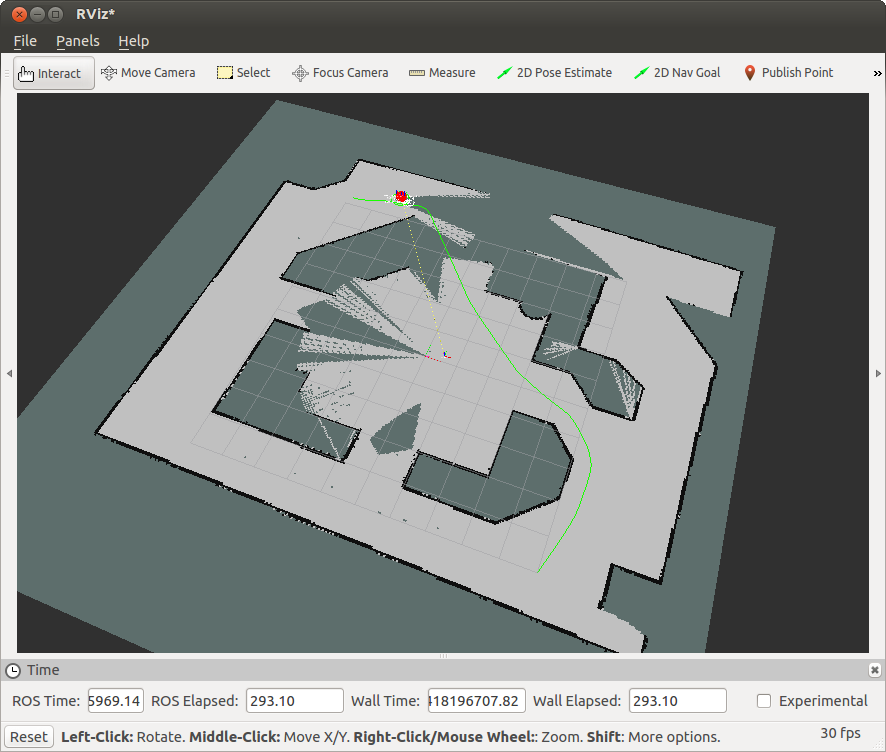
\includegraphics[width=\textwidth,height=\textheight,keepaspectratio]{img/navigation_simulation_rviz.png}
    \caption{rviz view}
  \end{subfigure}
  \begin{subfigure}[b]{0.8\textwidth}
    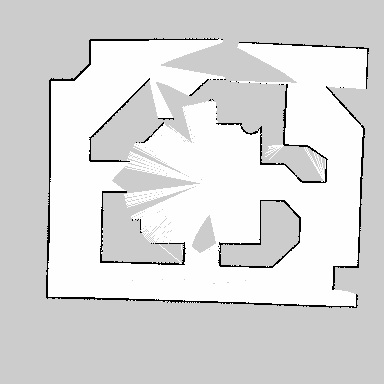
\includegraphics[width=\textwidth,height=\textheight,keepaspectratio]{img/gmapping_simulation_map.png}
    \caption{resulting map}
  \end{subfigure}
  \caption{Experiments in the simulator}
  \label{fig:navigationresults}
\end{figure}

\begin{figure}[h!]
  \centering
  \begin{subfigure}[b]{0.8\textwidth}
    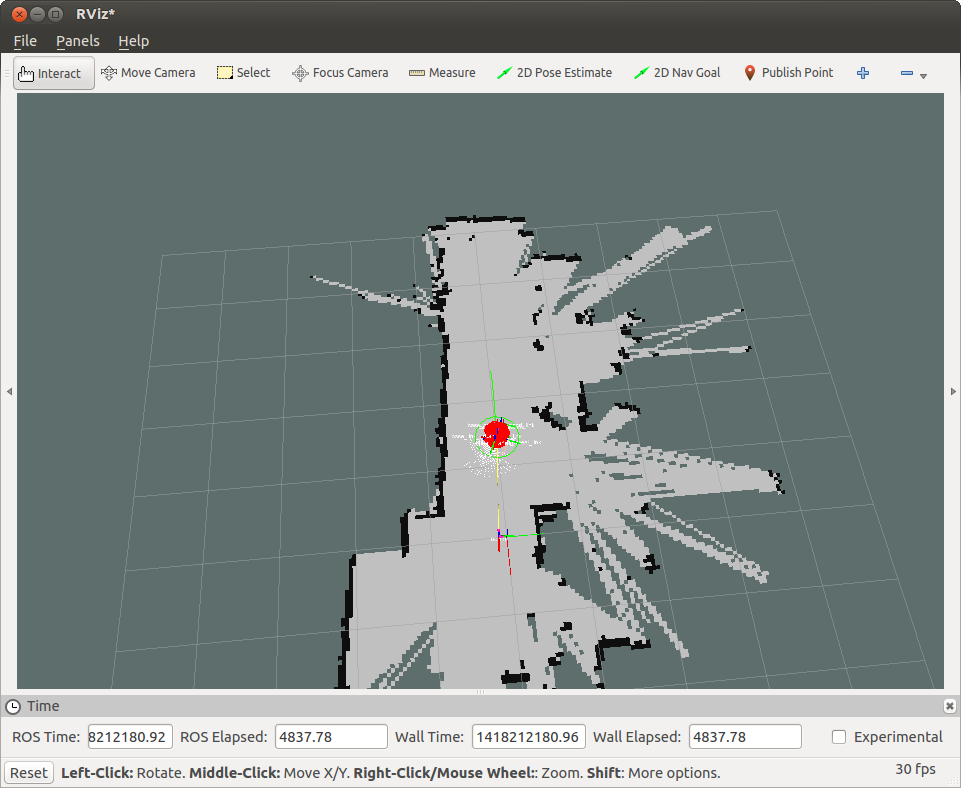
\includegraphics[width=\textwidth,height=\textheight,keepaspectratio]{img/navigation_real_rviz.png}
    \caption{rviz view}
  \end{subfigure}
  \begin{subfigure}[b]{0.8\textwidth}
    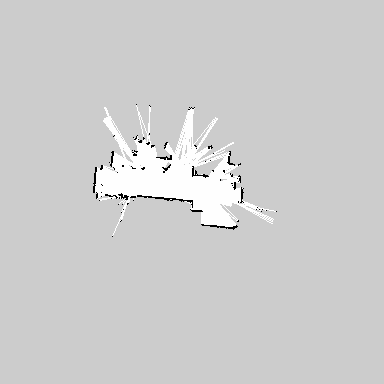
\includegraphics[width=\textwidth,height=\textheight,keepaspectratio]{img/gmapping_real_map.png}
    \caption{resulting map}
  \end{subfigure}
  \caption{Experiments in the real world}
  \label{fig:navigationresults}
\end{figure}


A sequence of images was recorded using the hector\_geotiff library.

\begin{lstlisting}[caption=Recording the map as generated by gmapping]
rosrun hector_trajectory_server hector_trajectory_server
rosrun hector_geotiff geotiff_node map:=dynamic_map
rostopic pub -r 1 /syscommand std_msgs/String "data: 'savegeotiff'"
\end{lstlisting}


\begin{figure}[h!]
  \centering
  \begin{subfigure}[b]{0.4\textwidth}
    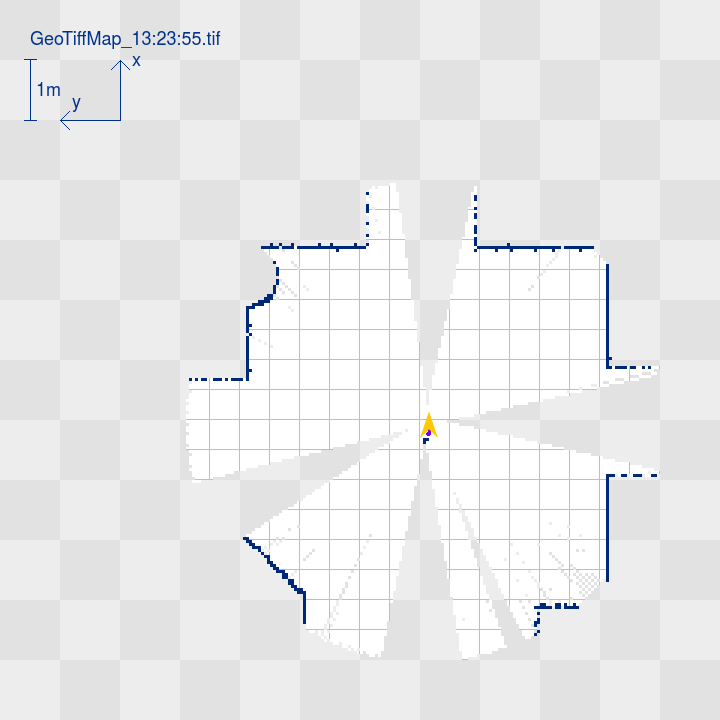
\includegraphics[width=\textwidth,height=\textheight,keepaspectratio]{img/move_square/1.png}
  \end{subfigure}
  \begin{subfigure}[b]{0.4\textwidth}
    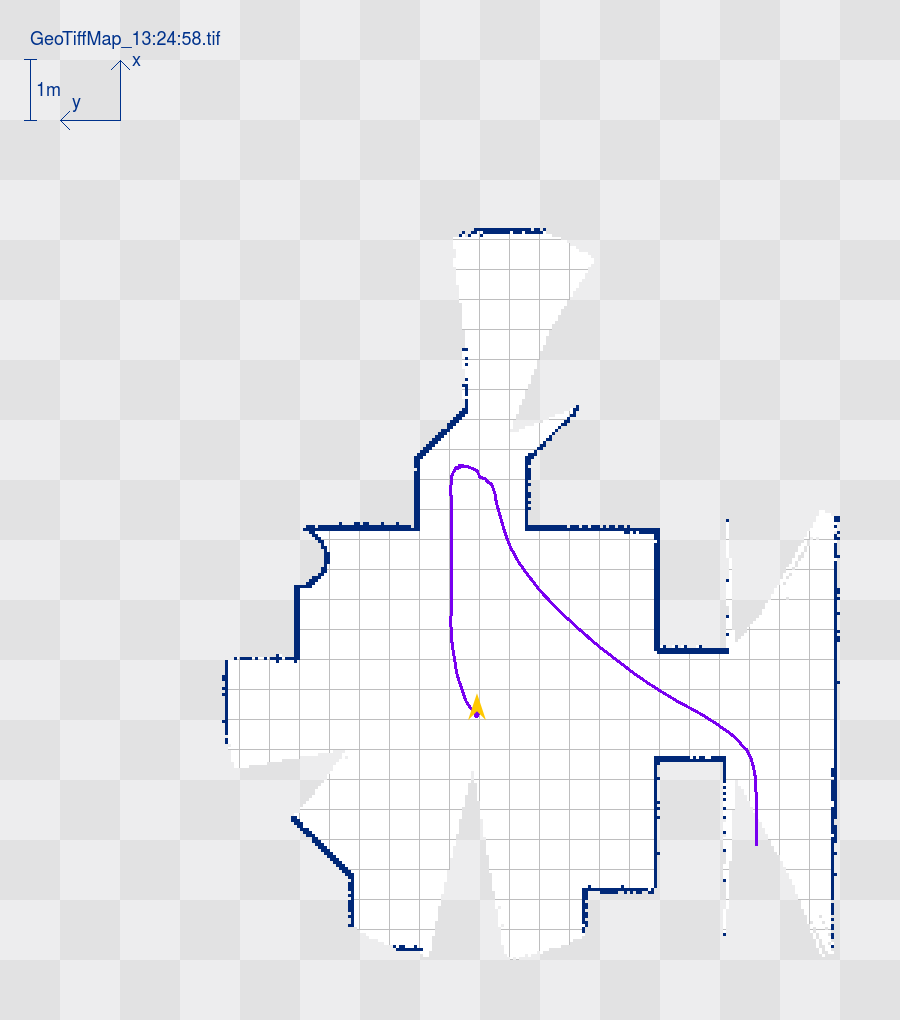
\includegraphics[width=\textwidth,height=\textheight,keepaspectratio]{img/move_square/2.png}
  \end{subfigure}
  \begin{subfigure}[b]{0.4\textwidth}
    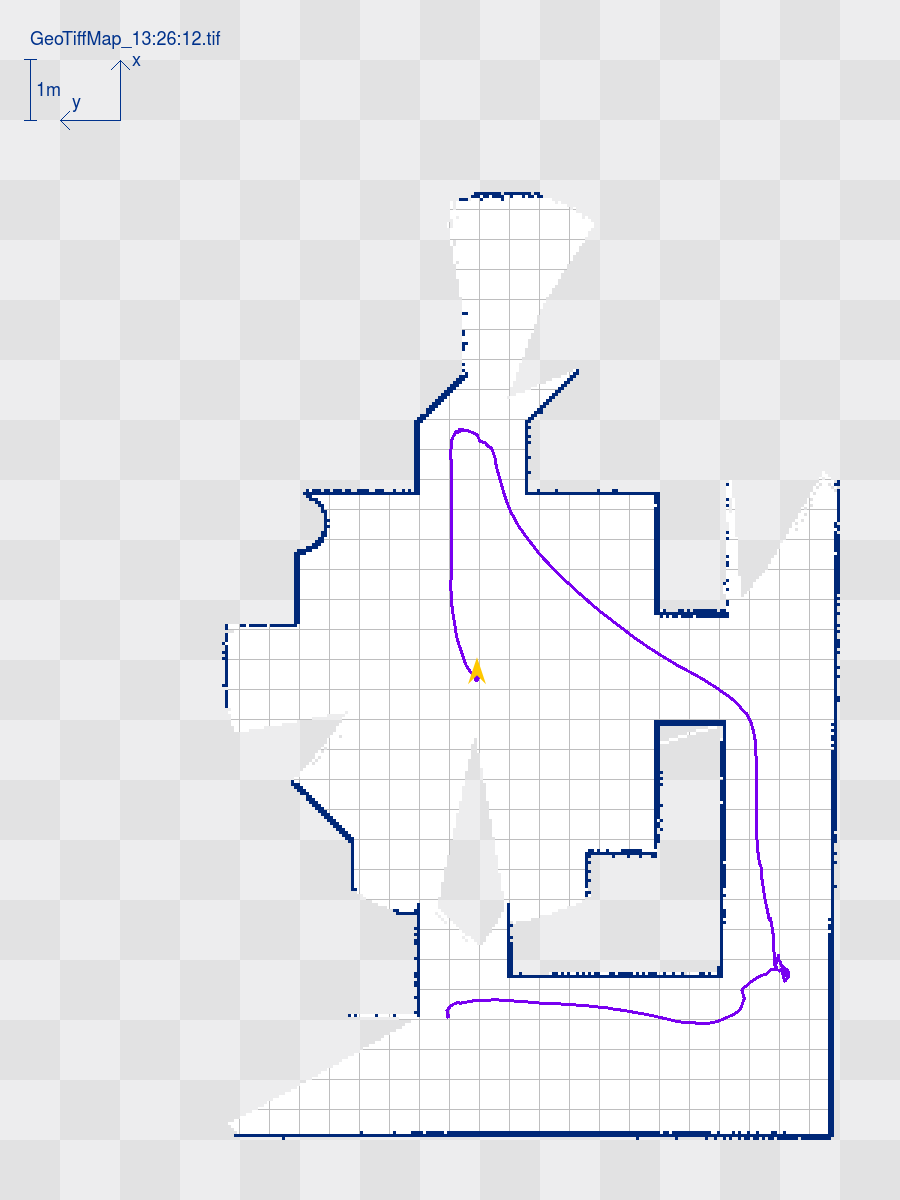
\includegraphics[width=\textwidth,height=\textheight,keepaspectratio]{img/move_square/3.png}
  \end{subfigure}
  \begin{subfigure}[b]{0.4\textwidth}
    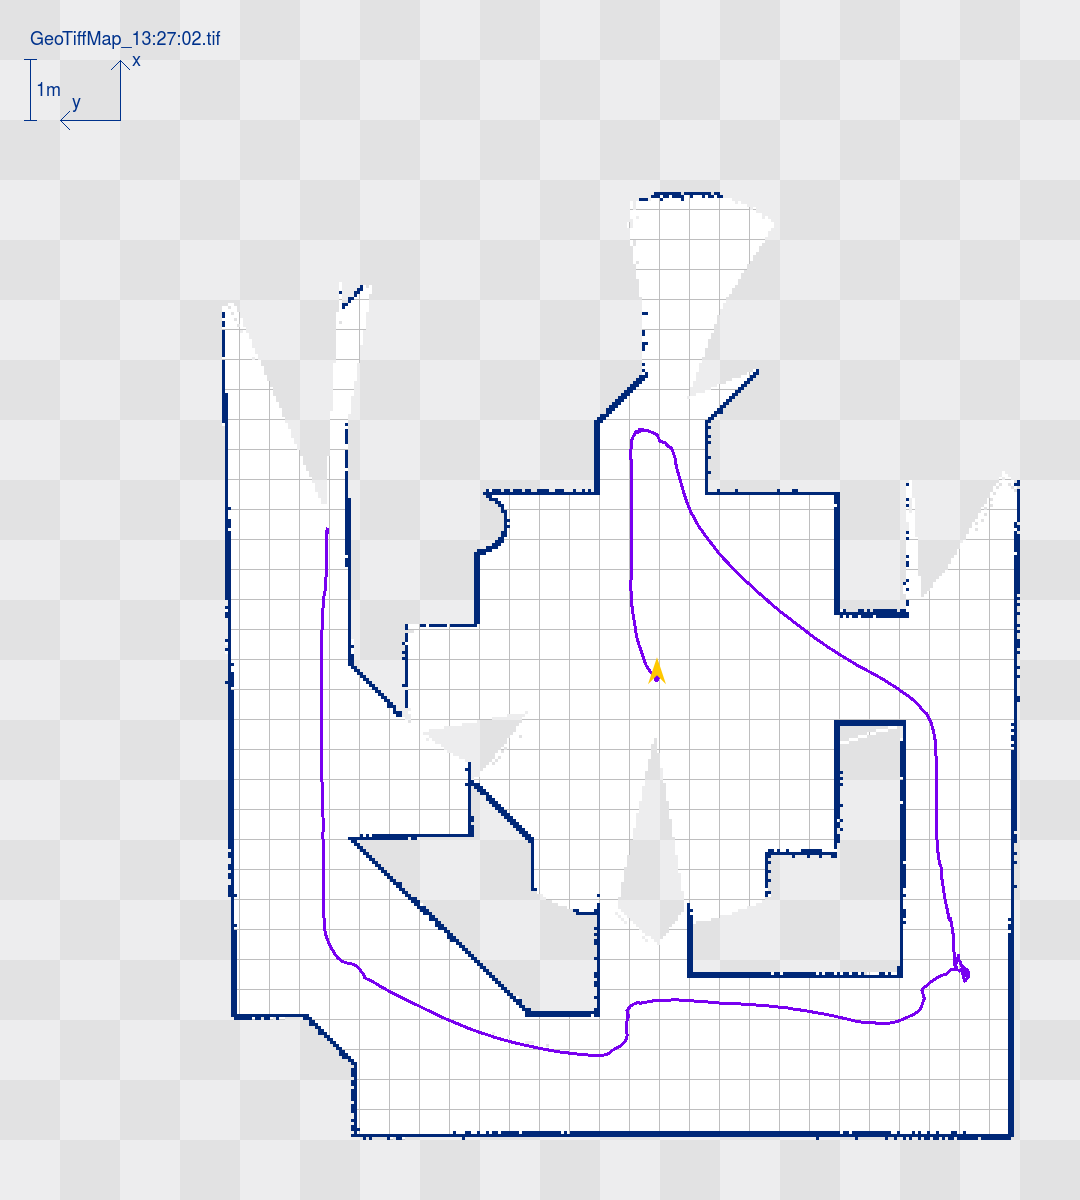
\includegraphics[width=\textwidth,height=\textheight,keepaspectratio]{img/move_square/4.png}
  \end{subfigure}
  \begin{subfigure}[b]{0.4\textwidth}
    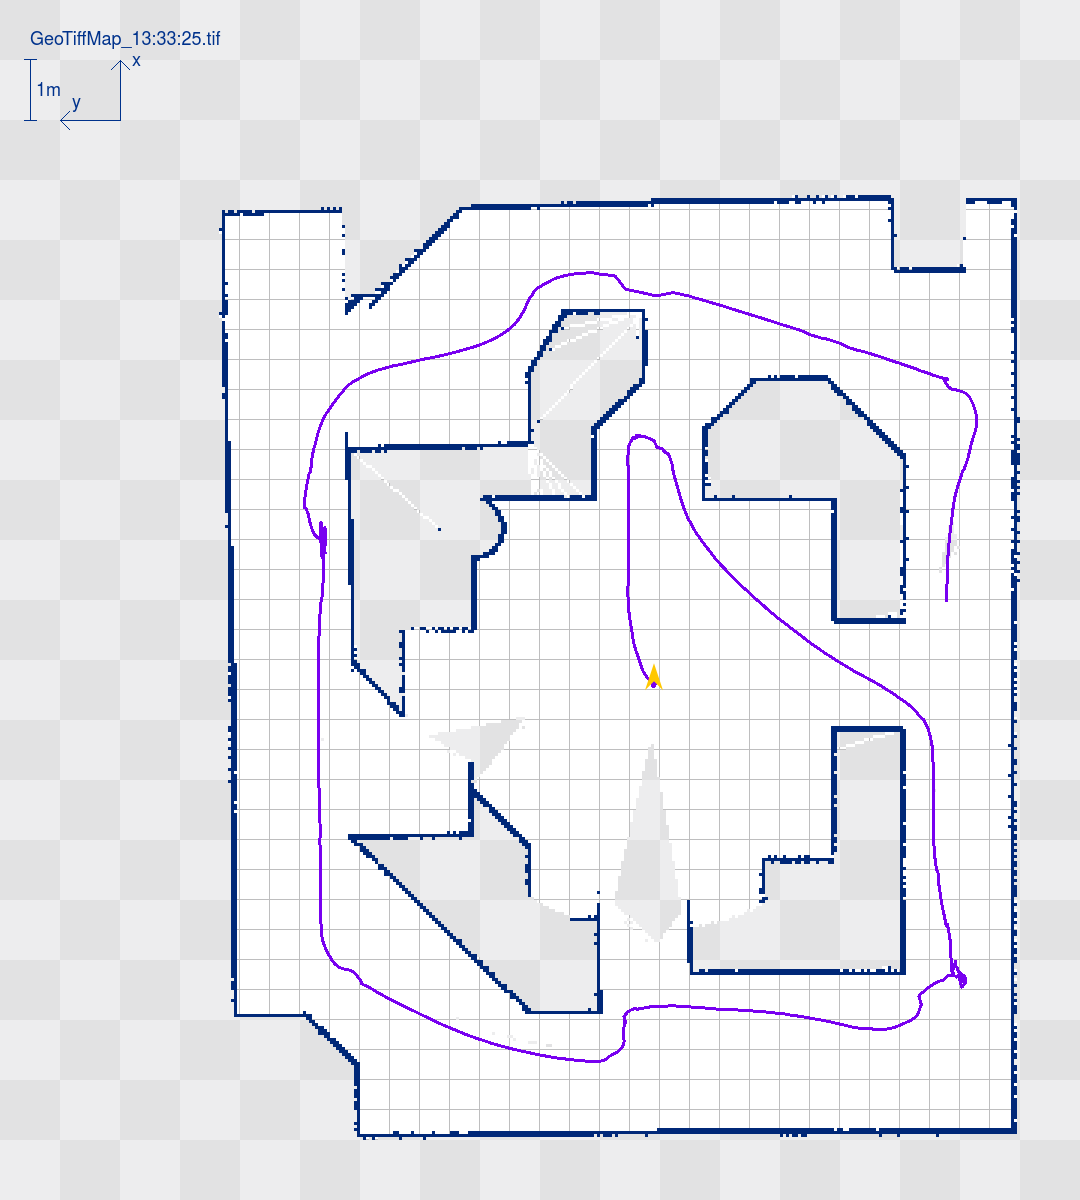
\includegraphics[width=\textwidth,height=\textheight,keepaspectratio]{img/move_square/5.png}
  \end{subfigure}
  \begin{subfigure}[b]{0.4\textwidth}
    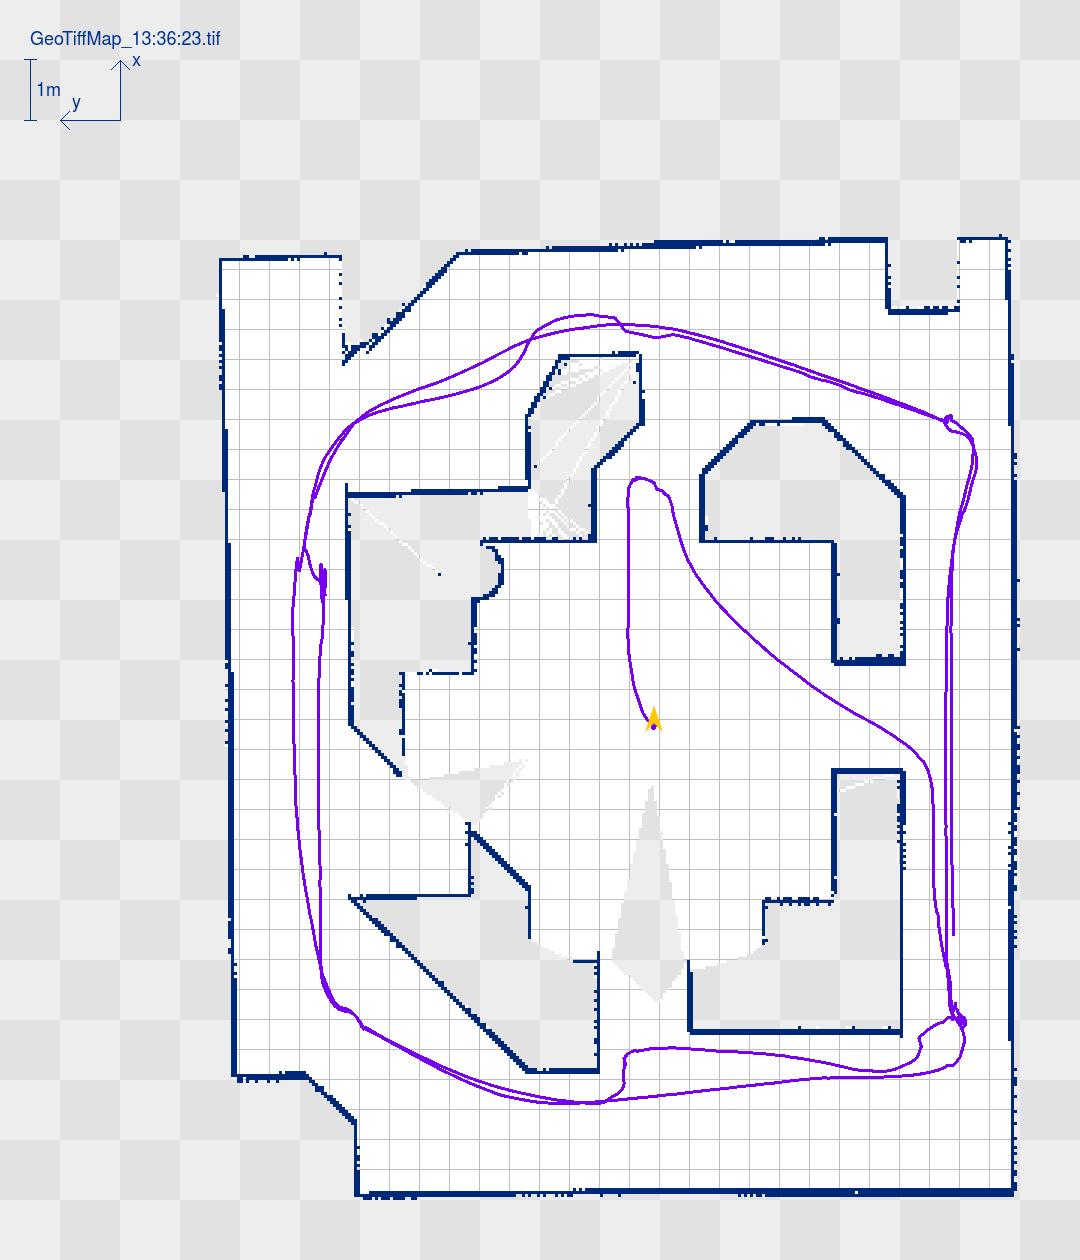
\includegraphics[width=\textwidth,height=\textheight,keepaspectratio]{img/move_square/6.png}
  \end{subfigure}
  \caption{Simulated robot exploration and planning}
\end{figure}


\subsection{Issues encountered}
\subsubsection{Extrapolation error}
An issue encountered was that when running the navigation software on the robot,
the move-base node reports an error:

\begin{lstlisting}[caption=Error message when running on different pc]
[ INFO] [1418207278.346072074]: Got new plan
[ERROR] [1418207278.346767687]: Extrapolation Error: Lookup would require extrapolation into the future.  Requested time 1418207278.408950434 but the latest data is at time 1418207278.374471708, when looking up transform from frame [odom] to frame [map]

[ERROR] [1418207278.346911345]: Global Frame: odom Plan Frame size 31: map

[ WARN] [1418207278.347037572]: Could not transform the global plan to the frame of the controller
[ERROR] [1418207278.347137469]: Could not get local plan
Registering Scans:Done
[ INFO] [1418207278.596014219]: Got new plan
\end{lstlisting}

The source of this error is that the time synchronization between the laptop and the pc is accurate enough.
One solution was to run all navigation software on the laptop on the robot.
Another solution is to always use the map frame. Usually the odom frame is used for local navigation,
but we can
use the map frame as well.

\section{Conclusions}
The odometry and the gmapping localization were realized on the x80sv platform.
The \rospackage{gmapping} package yields good results for mapping and positioning.
The move-base package was used to navigate the robot. Several alternative planners were
tried. The \rospackage{global-planner} package was the best global planner. The \rospackage{dwa-local-planner}
was the best evaluated local planner.


\section{Future work}

\begin{itemize}
  \item The skynav navigation stack could be transformed to work via the plugin system of
    move base ros package. The advantage is that this navigation stack is better suitable
    with move-base. The disadvantage is that the limitations of the move-base package will
    be encountered.
  \item The black box controller PCB could be replaced by a new design, which is simpler
    and contains a known controller for the wheels. This has the advantage that the
    controller is known and can be modified.
  \item The laptop on the robot should be replaced by an embedded solution, capable of
    running the navigation stack.
  \item The smooth-planner and ompl planner could be further fine-tuned and extended.
    This would result in a wider range of available planners, and thus more flexibility.
  \item As an alternative for gmapping, the hector-slam module and amcl \cite{amcl}
    could be tried as an alternative. It is now unknown what the capabilities of these
    modules are.
  \item The semantic processor should be implemented.
  \item The initial map and robot position problems should be implemented.
\end{itemize}

\appendix

\section{Demo manual}
To demo the robot with the navigation software, follow the following steps:

Launch the robot driver on the robot:
\begin{lstlisting}
roslaunch x80sv_bringup real_robot_driver.launch
\end{lstlisting}

Now open rqt and use the robot steering plugin to verify that the robot moves.

If the robot moves correctly, launch the navigation stack (either on the robot itself
or another laptop or PC in the case of ros multimaster mode):
\begin{lstlisting}
roslaunch x80sv_navigation x80sv_navigation.launch
\end{lstlisting}

Now open rviz and give a navigation goal by using the 2d nav goal tool in rviz.
To visualize different topics rviz, in the view panel click add, and add the robot
model, the laserscan message and the map.


\end{document}


